\documentclass[../thesis.tex]{subfiles}

\begin{document}

\chapter{Experiments}
\label{chap:exp}

\noindent In this chapter, we present the results from the experiments that were done in this thesis. The results are split into two sections, i.e. the results from the cluster analysis and the classification sub procedure mentioned in figure (\ref{fig:ML_proc_thesis}). For each of the sections we present an overview of the statistical problems that the algorithms are to solve. In this, we also present the assumptions and the evaluation criteria that are used to rank the algorithms given the statistical learning problem that they need to solve. 

\section{Cluster Analysis}

\noindent In the cluster analysis, we try to see how well the various clustering algorithms perform in producing phenotypically distinct clinical patient groups with HFpEF and HFmrEF. We will organize this section in the following way: we start out by looking at the full sample data set, i.e. \texttt{HFfullDataSet.Rdat}.  After the pre-processing, we will run the principal components that explain 95\% of the variance in the dataset thought the clustering algorithms. The idea is to see how well the clustering algorithms perform in producing patients groups that are more unique compared to the physicians evaluation. Our measure of success is the number of unique baseline characteristics that are statistically significant using the Person $\chi^2$ test for categorical variables, ANOVA for normally distributed variables and Kruskal–Wallis test for non-normally distributed variables \citep{kruskal1952use}. The implementation is done using the \texttt{multigrps}-function from the \texttt{CBCgrps}-package in \texttt{r} \citep{CBCgrps}. The algorithms are first going to be performed on the subtype estimation problem, i.e. see how unique the patient groups produced are given that the only HF subtypes in the dataset is HFmrEF and HFpEF. After this is done, we will see how well the algorithms will perform in producing new clusters within the already defined patient groups from the first round. We will do the same analysis on both the groups that have been defined by the physicians and the first round clustering results. 

\subsection{The Subtype Estimation HF Problem}

\subsection{Clustering Based on Post-Diagnosis}

\begin{figure}
    \centering
    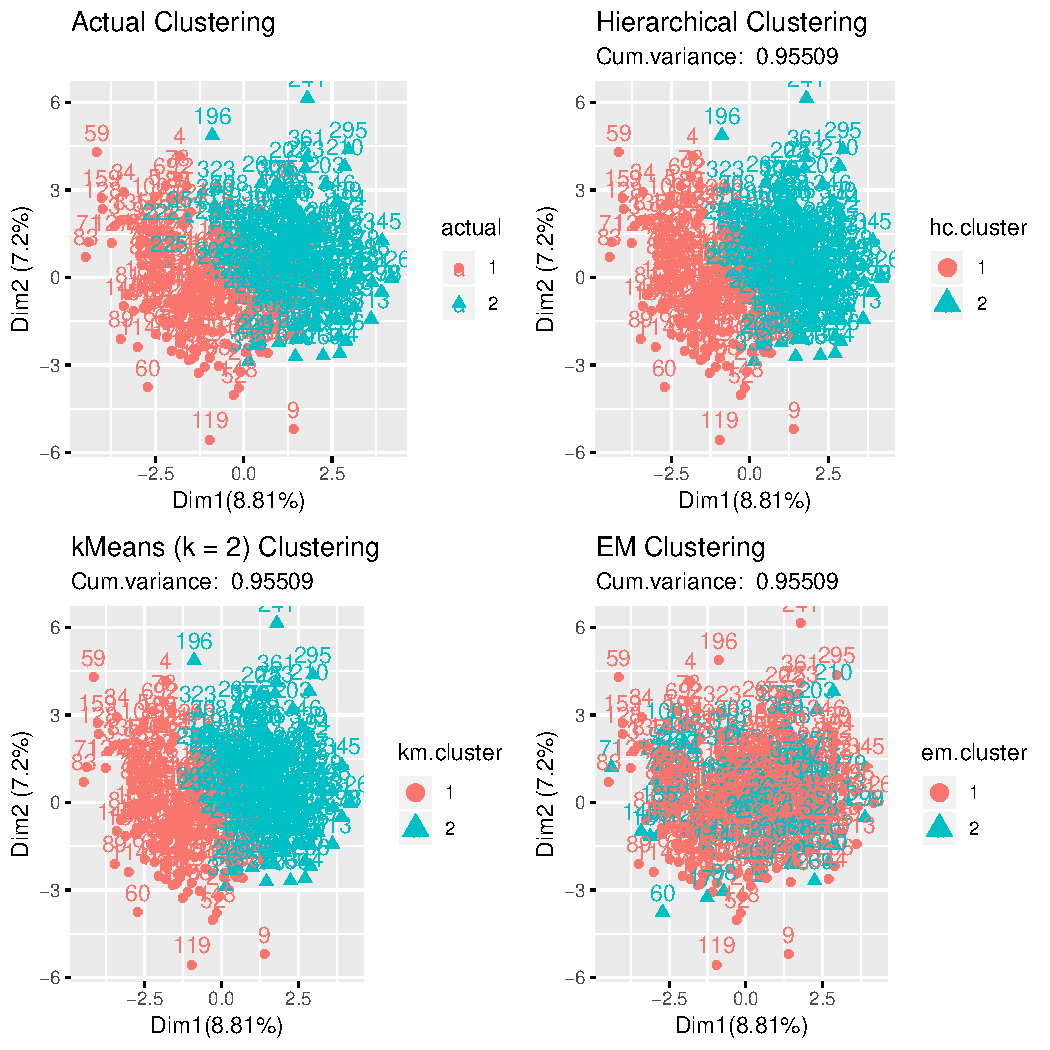
\includegraphics[width=1.15\textwidth]{doc/thesis/images/clustFull.pdf}
    \caption{\textit{Clustering with 31 principal components from subtype estimation}}
    \label{fig:clust_fulle}
\end{figure}

\subsection{Clustering Without Post-Diagnosis}

\section{Classification}

\subsection{Overview}

\subsection{Mortality Classifier}

\subsection{Re-admission Classifier}

\section{Discussion}

\end{document}